\documentclass{beamer}
% Use DS9 global theme (includes pgfplots for visualization)
\usepackage{../../../shared/templates/ds9_theme}

% Additional packages for code and visualization
\usepackage{listings}
\usepackage{tikz}
\usetikzlibrary{shapes, arrows, positioning, calc}
\usetikzlibrary{chains, positioning, scopes}


% Title page configuration
\title[Arrays in C++]{CS12 CH: Arrays and Memory Management}
\subtitle{Introduction to Contiguous Data Structures}
\author[Mr. Gullo]{Mr. Gullo}
\date[\today]{\today}

% Configure listings for C++ code
\lstset{
language=C++,
basicstyle=\ttfamily\small,
keywordstyle=\color{blue},
stringstyle=\color{green!60!black},
commentstyle=\color{gray}\itshape,
morecomment=[l][\color{magenta}]{#},
numbers=left,
numberstyle=\tiny\color{gray},
stepnumber=1,
breaklines=true,
tabsize=4,
showstringspaces=false,
frame=lines,
escapeinside={(@}{@)}
}

\begin{document}
\frame{\titlepage}

% -------------------------------------------------------------------------
% Learning Objectives
% -------------------------------------------------------------------------
\begin{frame}
\frametitle{Learning Objectives}
\begin{itemize}
\item \textbf{Define} an array as a contiguous memory structure for storing multiple values of the same type.
\item \textbf{Declare and Initialize} arrays using explicit sizing and initializer lists.
\item \textbf{Access and Modify} array elements using zero-based indexing.
\item \textbf{Implement} standard array algorithms including traversal, search, and aggregation (min/max).
\item \textbf{Identify} common pitfalls such as out-of-bounds access and off-by-one errors.
\end{itemize}
\end{frame}

% -------------------------------------------------------------------------
% Key Concepts
% -------------------------------------------------------------------------
\begin{frame}
\frametitle{Key Concepts: The Array}
\begin{block}{Definition}
An \textbf{array} is a collection of variables of the \textit{same type} that are referred to by a common name.
\end{block}

\vspace{0.5cm}

\textbf{Core Characteristics:}
\begin{itemize}
\item \textbf{Homogeneous}: All elements must be of the same data type (e.g., all \texttt{int} or all \texttt{float}).
\item \textbf{Contiguous}: Elements are stored in consecutive memory locations.
\item \textbf{Fixed Size}: In standard C++, the size of a stack-allocated array must be known at compile time and cannot change.
\item \textbf{Zero-Indexed}: The first element is always at index 
0
0
.
\end{itemize}
\end{frame}

% -------------------------------------------------------------------------
% Essential Syntax / Equations
% -------------------------------------------------------------------------
\begin{frame}
\frametitle{Essential Syntax and Logic}

\begin{block}{Declaration & Initialization}
\texttt{type name[size];}\
\texttt{int numbers[5] = {10, 20, 30, 40, 50};}
\end{block}

\begin{block}{Element Access}
\texttt{variable = arrayName[index];}\
\textit{Valid indices range from 
0
0
 to 
size−1
size−1
.}
\end{block}

\begin{block}{Memory Address Formula}
\texttt{Address of A[i] = BaseAddress + (i × sizeof(T))}

\vspace{0.3cm}
\textbf{Example:} \texttt{int scores[5];} starts at address \texttt{0x1000}
\begin{itemize}
    \item \texttt{scores[0]} → \texttt{0x1000 + (0 × 4)} = \texttt{0x1000}
    \item \texttt{scores[1]} → \texttt{0x1000 + (1 × 4)} = \texttt{0x1004}
    \item \texttt{scores[2]} → \texttt{0x1000 + (2 × 4)} = \texttt{0x1008}
\end{itemize}

\vspace{0.2cm}
\small{\textit{Note: 0x means hexadecimal (base-16). Each int is 4 bytes, so addresses increase by 4.}}
\end{block}

\end{frame}

% -------------------------------------------------------------------------
% Concept Visualization: Memory Layout (Context)
% -------------------------------------------------------------------------
\begin{frame}
\frametitle{Visualizing Memory: Contiguous Storage}
\textbf{How are arrays stored in RAM?}\pause

\vspace{0.5cm}

Unlike individual variables which may be scattered in memory, arrays claim a single, solid block of space.

\vspace{0.5cm}

\begin{itemize}
\item The \textbf{Array Name} represents the starting address (Base Pointer).
\item The \textbf{Index} represents the "offset" or distance from the start.
\item Because the size of each element is known (e.g., 4 bytes for an integer), the computer can instantly calculate the location of any element.
\end{itemize}

\vspace{0.5cm}

\textit{Next Slide: Visualization of \texttt{int myArr[5]} in memory.}
\end{frame}

% -------------------------------------------------------------------------
% Concept Visualization: Memory Layout (Diagram)
% -------------------------------------------------------------------------

\begin{frame}
\frametitle{Memory Layout Visualization}
\centering

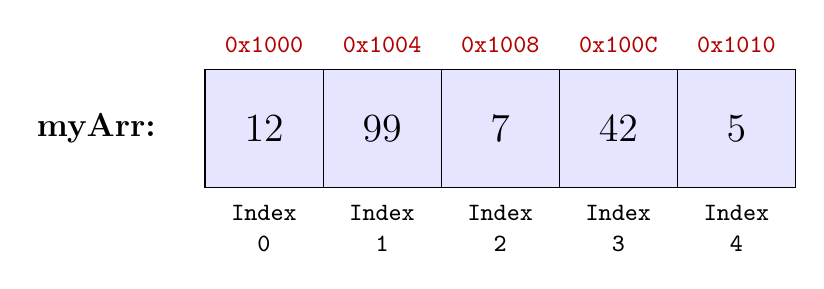
\begin{tikzpicture}[
    % 1. Start a chain going right
    start chain=1 going right,
    % 2. Set spacing to 0 so blocks touch
    node distance=0pt,
    % 3. Define styles
    memblock/.style={
        draw,
        rectangle,
        minimum width=1.5cm,
        minimum height=1.5cm,
        outer sep=0pt,      % Ensures lines overlap perfectly
        fill=blue!10,       % Simpler syntax for light blue
        font=\Large,
        on chain            % Automatically adds every memblock to the chain
    },
    label/.style={
        font=\small\ttfamily,
        align=center,
        color=black
    }
]

% --- Array Blocks ---
% Because 'on chain' is in the style, we just list the nodes
\node [memblock] (0) {12};
\node [memblock] (1) {99};
\node [memblock] (2) {7};
\node [memblock] (3) {42};
\node [memblock] (4) {5};

% --- Indices (Below) ---
% Using 'positioning' library syntax
\node [below=0.1cm of 0, label] {Index\\0};
\node [below=0.1cm of 1, label] {Index\\1};
\node [below=0.1cm of 2, label] {Index\\2};
\node [below=0.1cm of 3, label] {Index\\3};
\node [below=0.1cm of 4, label] {Index\\4};

% --- Addresses (Above) ---
\node [above=0.1cm of 0, label, color=red!70!black] {0x1000};
\node [above=0.1cm of 1, label, color=red!70!black] {0x1004};
\node [above=0.1cm of 2, label, color=red!70!black] {0x1008};
\node [above=0.1cm of 3, label, color=red!70!black] {0x100C};
\node [above=0.1cm of 4, label, color=red!70!black] {0x1010};

% --- Variable Label ---
\node [left=0.5cm of 0, font=\bfseries\large] {myArr:};

\end{tikzpicture}

\vspace{0.5cm}
\footnotesize
Notice: Addresses increase by 4 bytes per index.\\
\texttt{myArr[2]} is located at \texttt{0x1000 + (2 * 4) = 0x1008}.
\end{frame}

% -------------------------------------------------------------------------
% Code Example: Fundamentals (Part 1)
% -------------------------------------------------------------------------
\begin{frame}
\frametitle{Demo: Array Fundamentals}
\textbf{File:} \texttt{arrayIntro\_01.cpp}

\vspace{0.3cm}
\textbf{Operations demonstrated:}
\begin{enumerate}
    \item \textbf{Declaration \& Initialization} --- Create array with initializer list; compiler auto-determines size
    \item \textbf{Length Tracking} --- Use \texttt{const int length} to avoid magic numbers
    \item \textbf{Element Access} --- First element: \texttt{arr[0]}, Last element: \texttt{arr[length-1]}
    \item \textbf{Traversal} --- Loop through all elements using \texttt{for(int i = 0; i < length; i++)}
    \item \textbf{In-place Modification} --- Transform values directly: \texttt{arr[i] = arr[i] * arr[i]}
\end{enumerate}
\end{frame}

% -------------------------------------------------------------------------
% Code Example: Fundamentals (Part 2)
% -------------------------------------------------------------------------
\begin{frame}
\frametitle{Demo: Arrays and Functions}
\textbf{File:} \texttt{arrayIntro\_02.cpp}

\vspace{0.3cm}
\textbf{Operations demonstrated:}
\begin{enumerate}
    \item \textbf{Calculate Array Length} --- \texttt{sizeof(arr)/sizeof(arr[0])} returns number of elements
    \item \textbf{Declare Empty Array} --- \texttt{int arr[SIZE];} creates array of fixed size (uninitialized)
    \item \textbf{Fill with Computed Values} --- Use loop to populate: \texttt{arr[i] = 2*i}
    \item \textbf{Pass Array to Function} --- Arrays passed by reference automatically (no copy made)
    \item \textbf{Print Function} --- Helper function to display array contents with range parameters
\end{enumerate}
\end{frame}


% -------------------------------------------------------------------------
% Common Pitfalls
% -------------------------------------------------------------------------
\begin{frame}[fragile]
\frametitle{Warning: The Bounds Trap}
\textbf{File:} \texttt{arrayIntro_weird.cpp}

C++ does \textbf{not} check if you stay inside the array boundaries. Accessing \texttt{arr[10]} of a size-5 array is technically allowed by the compiler but causes \textbf{Undefined Behavior}.

\begin{lstlisting}
int aArr[] = {0, 1, 2, 3, 4}; // Size is 5
int bArr[] = {5, 6, 7, 8, 9};

// DANGEROUS: Accessing memory outside aArr
// This might print data from bArr, garbage, or crash the program
for(int i = 0; i < 12; i++) {
cout << aArr[i] << " ";
}
\end{lstlisting}

\alert{[Imagine reading past the end of the array into "unknown" memory territory]}
\end{frame}

% -------------------------------------------------------------------------
% Student Exercises: Intro
% -------------------------------------------------------------------------
\begin{frame}
\frametitle{Student Exercises}
\textbf{Goal:} Implement standard array utility functions.

\vspace{0.5cm}

\textbf{Exercise File:} \texttt{array_introduction_exercise.cpp}

\vspace{0.5cm}

You will complete the function bodies for:
\begin{enumerate}
\item \texttt{initializeArray}: Filling an array with values.
\item \texttt{randomArray}: Generating random data.
\item \texttt{arrayMaximum}: Finding the largest value.
\item \texttt{reverseArray}: Modifying the order of elements.
\end{enumerate}

\vspace{0.2cm}
\textit{Open the file and locate the TODO sections.}
\end{frame}


% -------------------------------------------------------------------------
% Summary
% -------------------------------------------------------------------------
\begin{frame}
\frametitle{Summary}
\begin{itemize}
\item \textbf{Arrays} allow efficient storage of lists of data using contiguous memory.
\item \textbf{Indexing} starts at 0. The last valid index is always 
size−1
size−1
.
\item \textbf{Memory}: Arrays are just pointers to the start of a memory block.
\item \textbf{Safety}: You must manually ensure you do not read or write past the end of the array.
\item \textbf{Practice}: Mastering loops (for/while) is essential for effective array manipulation.
\end{itemize}
\end{frame}

\end{document}